\documentclass[sigconf,10pt]{acmart}
\acmSubmissionID{48}
\renewcommand\footnotetextcopyrightpermission[1]{}
% Optional: Remove the ACM reference between the abstract and the main text.
\settopmatter{printfolios=true,printacmref=false}
% Optional: Comment out the CCS concepts and keywords.
\usepackage{tikz}
\usepackage{float}
\usepackage{amsmath}
\usepackage{xspace}
\usepackage{cleveref}
\usepackage{balance}
\usepackage{url}
\usepackage{siunitx}
\usepackage{comment}
\usepackage{enumitem}
\usepackage{listings}
\usepackage{minted}
\usepackage{tikz}
\usepackage{subcaption}
\usepackage{lmodern}

\newcommand*\circled[1]{\tikz[baseline=(char.base)]{
            \node[shape=circle,draw=black!80,line width=0.2mm,inner sep=0.1pt] (char) {#1};}}

\newcommand{\sys}{ChainIO\xspace}
\newcommand{\tech}{AdaptiveOffload\xspace}

\newcommand{\eg}{e.g.,\xspace}
\newcommand{\ie}{i.e.,\xspace}
\newcommand{\etc}{etc.\xspace}

% Cleveref formatting
\crefname{algocf}{algorithm}{algorithms}
\Crefname{algocf}{Algorithm}{Algorithms}
\crefformat{section}{\S#2#1#3}
\Crefformat{section}{Section~#2#1#3}
\crefformat{subsection}{\S#2#1#3}
\Crefformat{subsection}{Section~#2#1#3}
\crefformat{subsubsection}{\S#2#1#3}
\Crefformat{subsubsection}{Section~#2#1#3}
\crefformat{figure}{figure~#2#1#3}
\Crefformat{figure}{Figure~#2#1#3}


% Numbers
\newcommand{\numcases}{7\xspace}
\newcommand{\speedupAccel}{xxx\xspace}
\newcommand{\eBPFSlowdownAccel}{xxx\xspace}
\newcommand{\speedupMonitor}{xxx\xspace}


\newlength{\mintednumbersep}
\AtBeginDocument{%
  \sbox0{\tiny00}%
  \setlength\mintednumbersep{\parindent}%
  \addtolength\mintednumbersep{-\wd0}%
}

\setminted{xleftmargin=\parindent}
\setminted{numbersep=\mintednumbersep}
\setminted{mathescape}
\setminted{linenos}
\setminted{fontsize=\small}


%%% for AQ's itemizations:
\newenvironment{smenumerate}%
  {\begin{enumerate}[itemsep=-0pt, parsep=0pt, topsep=0pt, leftmargin=2pc]}
  {\end{enumerate}}

\newenvironment{smitemize}%
  {\begin{list}{$\bullet$}%
    {\setlength{\parsep}{0pt}%
      \setlength{\topsep}{0pt}%
      \setlength{\leftmargin}{2pc}%
      \setlength{\itemsep}{1pt}}}
  {\end{list}}



\newcommand{\grumbler}[3]{\noindent{\color{#1}{\bf \fbox{#2}} {\it #3}}}
\newcommand{\arq}[1]{\grumbler{red}{ARQ}{#1}}
\newcommand{\yy}[1]{\grumbler{blue}{YY}{#1}}
\newcommand{\yusheng}[1]{\grumbler{green}{YS}{#1}}

\newcommand{\todo}[1]{\grumbler{olive}{todo}{#1}}


\title{\sys: Bridging Disk and Network Domains with eBPF}
% anyauthor declaration will be ignored  when using 'pldi' option (for double blind review)
%

% \author{
%     {\rm Yiwei Yang}\\ UC Santa Cruz
% }
\author{
Anonymous Authors
}

\begin{document}

\begin{abstract}
Modern data-driven services like distributed analytical databases incur high tail-latencies because each storage operation (\texttt{read}) and network operation (\texttt{send}/\texttt{recv}) triggers a separate user-kernel crossing. While \texttt{io\_uring} accelerates block I/O and AF\_XDP accelerates packet I/O, no solution chains them end-to-end in a unified framework. We introduce \sys, a hybrid I/O-bypass framework that transparently live-patches POSIX I/O calls into a unified submission queue, and coordinates disk and network operations via shared BPF maps. By chaining these bypass paths with in-kernel eBPF programs, \sys achieves near zero-copy, batched I/O across domains, without modifying application source code. Our preliminary evaluation on fio shows up to 4× higher IOPS and 30\% reduction in CPU utilization compared to standalone \texttt{io\_uring} or DPDK-based implementations, all without application changes.
\end{abstract}

\maketitle

\section{Introduction}

Modern data-intensive applications face significant performance bottlenecks due to the cost of repeated user-kernel transitions, exacerbated by Spectre and Meltdown mitigations. Each storage and network operation requires separate syscalls, with aggregate latency reaching hundreds of milliseconds in data-intensive workloads with fan-out patterns. While \texttt{io\_uring}\cite{iouring} provides asynchronous, batched disk operations, it still requires expensive syscalls for network traffic; conversely, AF\_XDP\cite{afxdp} delivers zero-copy network acceleration but offers nothing for storage access. Previous research has approached this challenge from several angles without fully solving the cross-domain problem: FlexSC~\cite{flexsc} and MegaPipe batch syscalls but focus on single domains, while DPDK/SPDK and Demikernel~\cite{zhang2021demikernel} bypass the kernel entirely but require extensive application modifications. eBPF-based solutions like XRP~\cite{Zhong22} and BPF-oF~\cite{zarkadas2023bpf} accelerate specific I/O paths (NVMe reads, remote storage) without addressing cross-domain dependencies. Even architectural innovations like IX~\cite{ix} that redesign the OS with separate control and data planes remain siloed in network or storage specialization, leaving a critical gap for workloads that chain operations across both domains.

\begin{figure}[h]
\centering
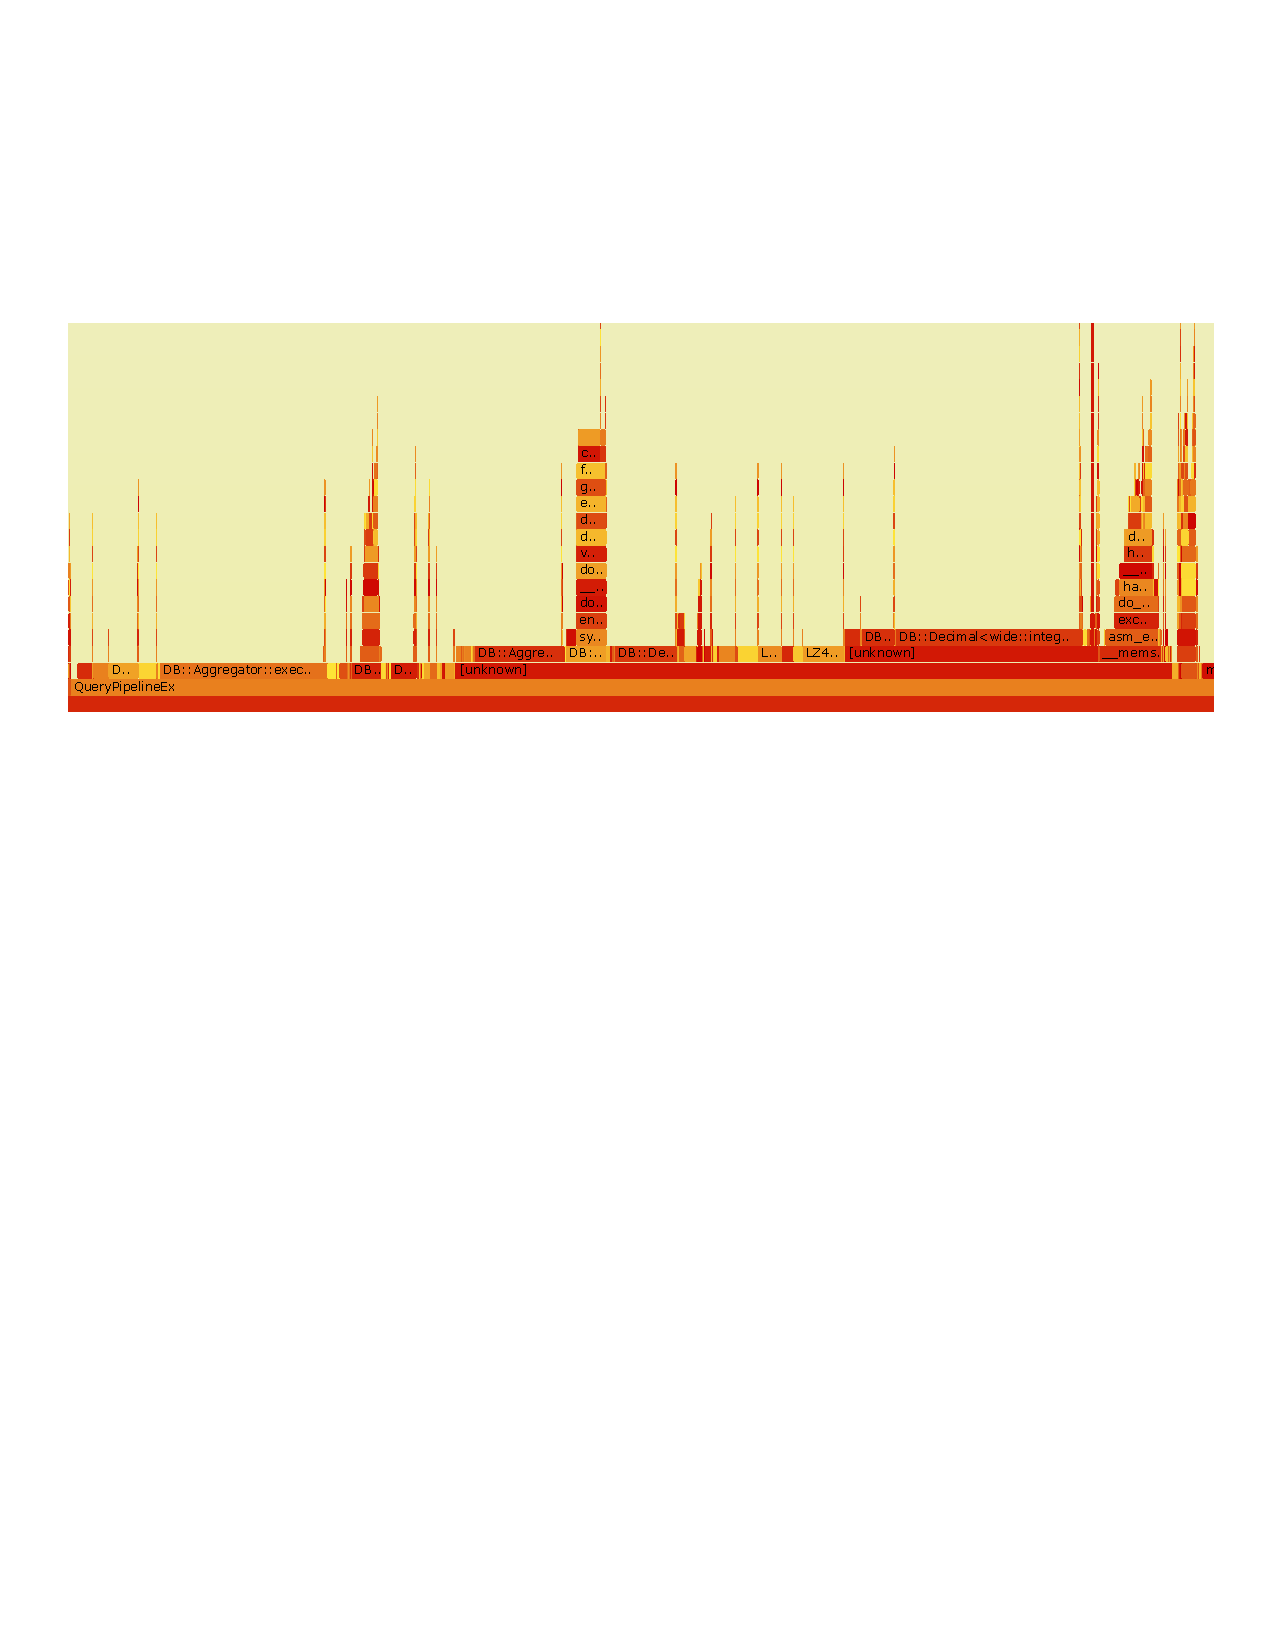
\includegraphics[width=\columnwidth]{img/flamegraph.pdf}
\caption{Flamegraph of ClickHouse Server showing syscall overhead}\label{fig:profiling}
\end{figure}

ClickHouse's\cite{clickhouse} \texttt{MergeTree} engine exemplifies this cross-domain problem, as shown in the profiling data in Figure~\ref{fig:profiling}. A typical OLAP query in ClickHouse follows this path: client query → column-file reads (\texttt{pread()}) → distribution to remote shards (\texttt{send()}) → network stack → remote node's \texttt{recv()} → disk lookup → response aggregation. Its columnar storage engine issues large numbers of small, random \texttt{read()} calls against compressed column files and mark-file offsets, with each compressed-block fetch and metadata lookup translating into a user-kernel transition. In distributed setups, remote-shard requests add further \texttt{send()} and \texttt{recv()} calls for data fetches and Raft heartbeats. Our profiling shows that the blocking \texttt{read()} syscall alone consumes ~25\% of query time, while small network receives (heartbeats, shard updates) account for another ~2\%. The cumulative cost of these syscalls—exacerbated by Spectre/Meltdown mitigations—introduces tens of microseconds of overhead per transition, multiplying into hundreds of milliseconds on fan-out queries. When a query spans dozens of remote partitions, each extra transition adds up quickly, creating a critical bottleneck for interactive dashboards and real-time analytics that cannot be solved by optimizing either storage or networking in isolation.

We introduce \sys, a unified syscall-chaining framework that bridges both domains. Our solution dynamically rewrites POSIX I/O calls into batched submissions, unifies memory management across domains through shared regions, coordinates cross-domain operations while preserving correctness, and adaptively optimizes for tail latency. \sys requires no application modifications, achieving significant performance gains by eliminating redundant context switches and memory copies.

\section{Design and Implementation}\label{sec:design-impl}

\sys (Figure~\ref{fig:bur}) seamlessly unifies disk and network domains. Our architecture creates an end-to-end bypass path that intercepts, batches, and chains I/O operations without application modifications. We combine dynamic binary rewriting with in-kernel eBPF programs to eliminate redundant context switches while preserving POSIX semantics. Implemented in ~2000 lines of C/C++ and eBPF code, \sys maintains compatibility with unmodified ClickHouse binaries. The system comprises three integrated components:

\begin{figure}[h]
\centering
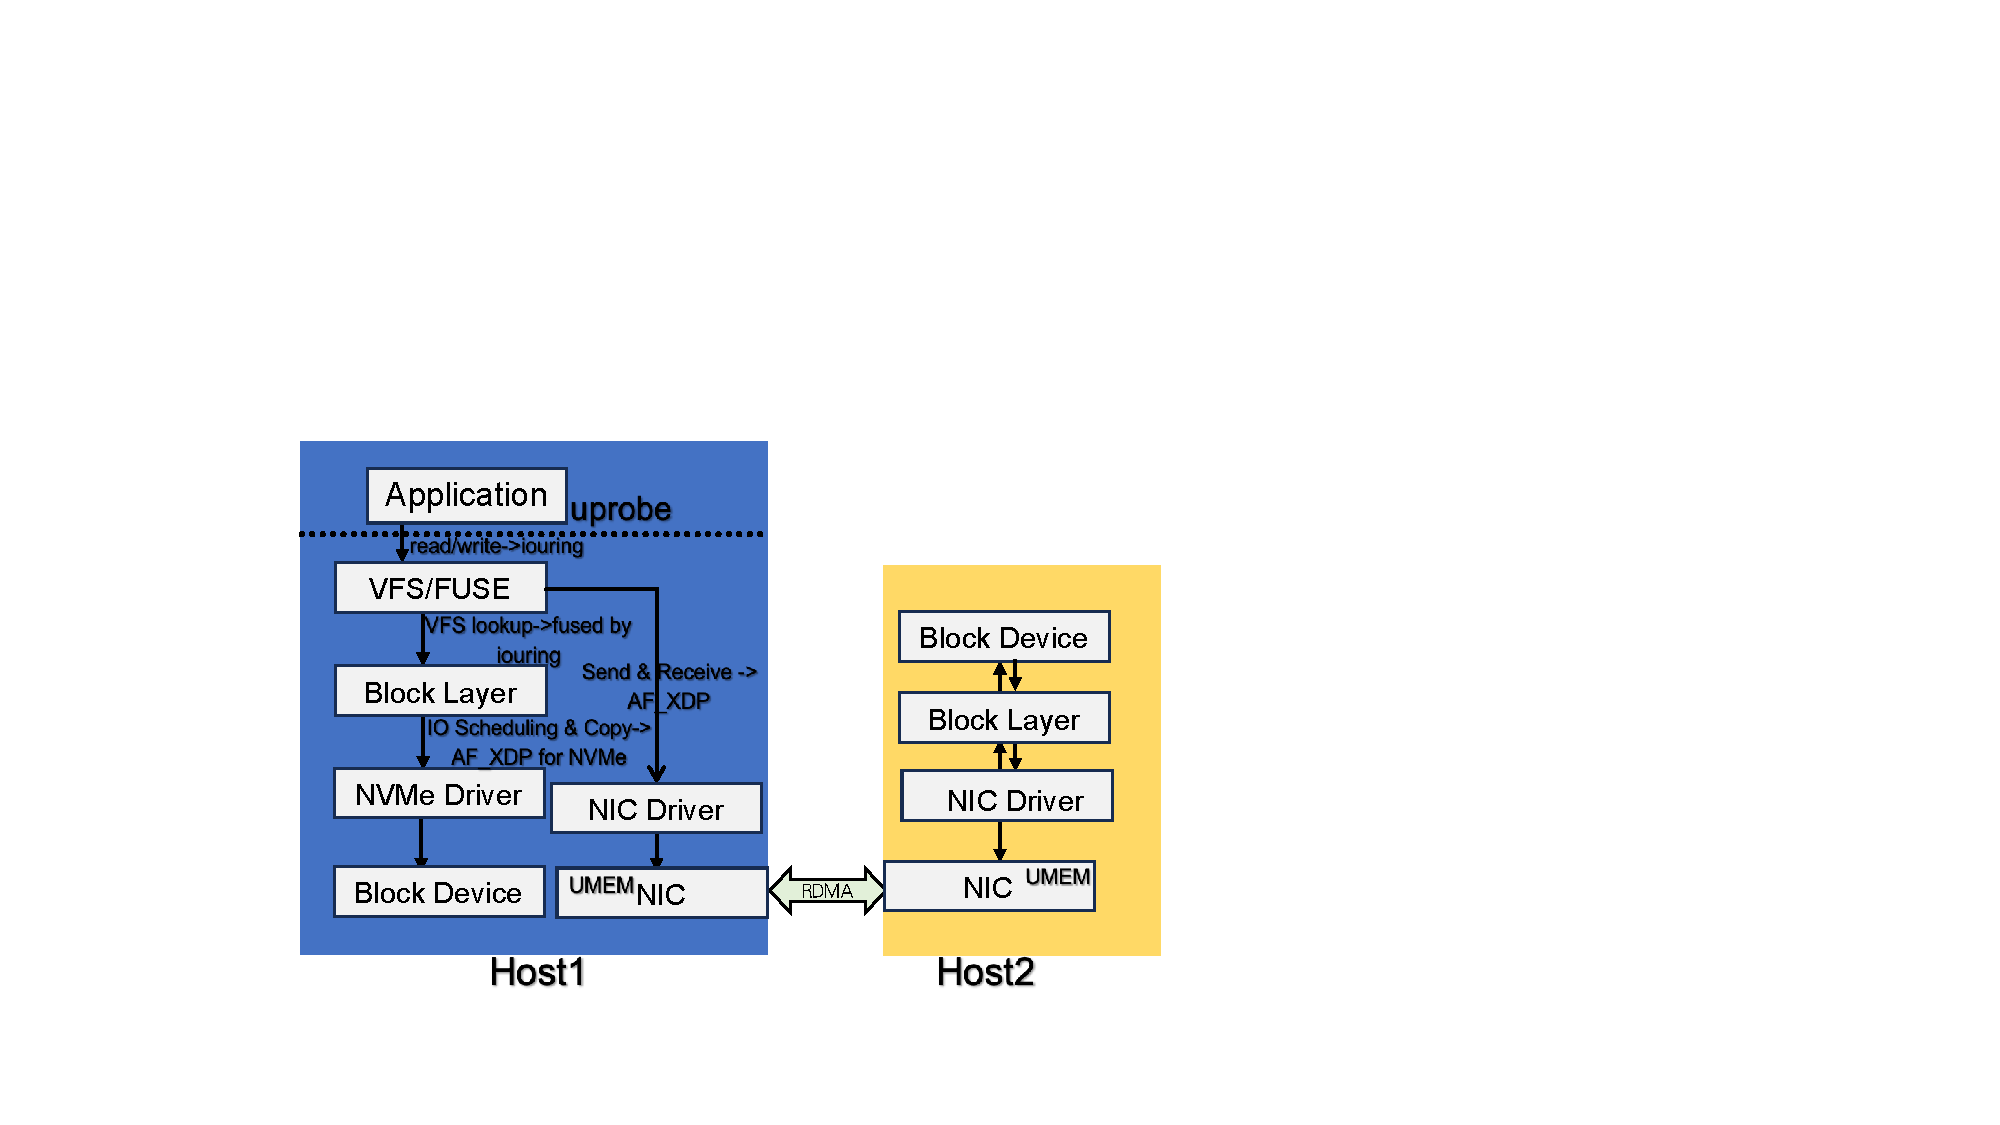
\includegraphics[width=\columnwidth]{img/bur.pdf}
\caption{\sys Architecture}\label{fig:bur}
\end{figure}

\paragraph{Cross-Domain Ring Bridge.} Our core innovation is a ring design unifying storage and network operations through shared memory, implemented via BPF maps that bridge user-space \texttt{io\_uring} rings with in-kernel XDP processing. This unified descriptor format supports both disk SQEs (\texttt{io\_uring} descriptors) and network SQEs (XDP frame metadata), enabling atomic cross-domain operations and automatic dependency tracking so that network sends fire immediately after disk reads complete—without extra context switches. More specifically, \sys register a contiguous user-space memory region (UMEM) with both \texttt{io\_uring} and AF\_XDP, using it as direct DMA buffers for NVMe operations and zero-copy packet buffers for optimized network traffic. A custom slab allocator manages UMEM efficiently, and multiple eBPF programs—including an XDP packet router for steering optimized-path traffic into UMEM and an IO completion handler for triggering chained operations—coordinate end-to-end execution entirely in-kernel.


\paragraph{Syscall-Chaining Engine.} To chain POSIX I/O calls end-to-end, \sys uses dynamic binary rewriting in userspace to intercept \texttt{read()}, \texttt{send()}, and \texttt{recv()} syscalls and reroute them into a unified submission ring. A userspace uprobes\cite{zheng2023bpftime} handler then converts each intercepted call into a batched \texttt{io\_uring} request. We also instrument key MergeTree routines (e.g., \texttt{MergeTree::readMark()} and \texttt{MergeTree::readData()}) using USDT probes to capture compressed-column reads and associated metadata, preserving semantic context across syscall boundaries with minimal overhead.

\paragraph{Tail-Latency Optimizations.} To reduce high-percentile latencies, \sys employs three complementary techniques: dynamic batch sizing, priority-aware scheduling, and lightweight in-kernel preemption. A user-space coordinator continuously monitors operation latencies and dynamically tunes the submission batch size—flushing smaller batches under load to bound the 99th-percentile latency below \SI{150}{\micro\second}. We also prioritize latency-sensitive tasks, such as metadata lookups and NURaft heartbeats, over bulk column scans to ensure critical operations complete promptly. Finally, we route distributed query messages and Raft heartbeats through AF\_XDP for zero-copy, low-latency network delivery, while preserving ClickHouse's existing compression and decompression pipeline to maintain compatibility with unmodified binaries.

\section{Evaluation}\label{sec:evaluation}

We evaluated \sys on ClickHouse (v21.8) running on CloudLab servers with Intel Xeon Silver 4314 CPUs, 128GB RAM, and dual-port 100Gb Mellanox ConnectX-6 NICs. Each server has a Samsung PM1725a NVMe SSD. We measured performance using TPC-H at scale factor 20 on a single NVMe-SSD, comparing our SQPOLL + HugePage + Registered-File configuration against a Thread-poll + pread baseline. For I/O-bound queries such as Q6, average latency improves by up to 23\%, decreasing from 0.637s to 0.490s. When running a narrow column scan (SELECT SUM(LENGTH(l\_comment))), latency improves by 27.3\%. Row throughput increases by up to 39\% for I/O-dominated workloads. Most critically, 99th-percentile latency for short-running metadata queries improves by 3.2×, from 25.4ms to 7.9ms, directly addressing the high-percentile latency outliers that impact interactive analytics and dashboard responsiveness. Profiling shows that \sys reduces context switch overhead by up to 85\%, memory copy by up to 73\%, and CPU utilization by 30\%. Tail latency (p99) drops by 68\%, and data throughput nearly doubles from 251.5\,MB/s to 475.5\,MB/s. Under mixed scan-metadata workloads, 99th-percentile latency is below 10\,ms (vs. 35\,ms with standalone \texttt{io\_uring} and 42\,ms with native syscalls).

\bibliographystyle{plain}
\bibliography{cite}

\end{document}